\documentclass{article}
\usepackage[utf8]{inputenc}
\usepackage{graphics}
\usepackage{graphicx}
\usepackage[francais]{babel}
\usepackage[T1]{fontenc} 



\begin{document}
\begin{flushright}

\includegraphics[scale = 0.2]{upmc.png}
\end{flushright}

\begin{center}
\par\vspace {2.5cm}
{\Huge\textbf{Cahier des charges : Hanabi\\*[0.25cm]}}   
\par\vspace {2cm}
{\Large\textbf{Université Pierre et Marie Curie\\ Projet ANDROIDE\\
               2015-2016}}                   
\par\vspace {2cm}
{\Large{Antunes Costa Gonçalves Daniel}}\\
{\Large{Assmann Catalina}}\\ 
{\Large{Hubert Cédric}}\\ 
{\Large{Wolfrom Matthieu}}\\
\end{center}

\newpage
\section{Présentation du projet}

\subsection{Contexte}

Ce projet se déroule dans le contexte de l’UE Projet de première année de Master ANDROIDE de l’UPMC.  Nous sommes un groupe de quatre étudiants qui doit mener à terme un projet proposé par leurs encadrants. Ce projet repose sur l’utilisation d’une intelligence artificielle qui exploite la logique épistémique afin d’appliquer la meilleure stratégie possible pour le jeu Hanabi. 
\subsection{Présentation du jeu Hanabi}

Hanabi est un jeu de cartes coopératif composé d'un ensemble de cartes et de jetons. Les cartes représentent des feux d'artifice et les joueurs doivent collaborer afin de composer cinq feux d'artifice de couleur différente. On dispose au début de la partie de 8 jetons <<indice>> qui représentent le nombre d'indices auquel on a encore le droit, ainsi que 3 jetons <<éclair>> qui représentent le nombre d'erreur que l'on peut faire avant de perdre la partie. Les jetons sont retournés lorsqu'un indice est donné ou une erreur commise. Un jeton d'indice peut être remis sur son côté initial lorsqu'on défausse une carte.   

Personne ne connaît ses propres cartes, mais chacun voit les cartes des autres. En utilisant des indices et les cartes visibles, les joueurs doivent essayer de poser les feux d'artifice en suites croissantes de cartes de même couleur.

Le score final est la somme des valeurs des dernières cartes posées pour chaque couleur.

Pour réussir ce défi, chaque joueur peut à son tour soit donner un indice à un autre joueur, soit défausser une carte, soit jouer une carte. 

Un indice consiste à indiquer quelles cartes sont d'une certaine couleur ou d'une certaine valeur. Un indice négatif peut aussi être donné, indiquant qu'un joueur ne possède aucune carte d'une certaine couleur ou valeur. À chaque indice, un jeton <<indice>> est utilisé et donc retourné. Si le joueur choisit de défausser une carte, il regagne un jeton <<indice>>. Par contre, quand un joueur tente sa chance et joue une carte, il est possible que la carte ne complète pas la suite de sa couleur de feu d'artifice, dans ce cas un jeton <<éclair>> est retourné. Une fois que trois jetons éclairs sont retournés, le jeu est fini et les joueurs ont perdu.


\subsection{Objectifs}

L’objectif de ce projet est de créer un logiciel qui permet à un joueur humain de jouer à Hanabi avec une ou plusieurs intelligences artificielles (maximum quatre). Nous allons proposer plusieurs modes de jeu :\\

 Facile :

\begin{itemize}

 \item Avec ou sans jetons
 \item Avec toutes les cartes visibles
 
\end{itemize}

 Normal :

\begin{itemize}

 \item Avec deux à cinq joueurs, toujours au plus un joueur humain. Pour une partie entre 2 ou 3 joueurs, chaque joueur a 5 cartes. Pour plus de joueurs, chaque joueur a 4 cartes.
 \item Avec toutes les IAs partageant la même stratégie ou avec des stratégies différentes.\\
 L’utilisateur peut y jouer via une interface graphique qui lui permettra de voir les cartes de son équipe, mais pas les siennes. 
 
\end{itemize}

Il y aura des options pour sauvegarder sa partie et la continuer ultérieurement. 

\subsection{Description de l'existant}

Le logiciel est réalisé avec le langage Java, et est déployable sous les principales plateformes le supportant. Nous l'avons choisi car c'est un langage orienté objet et donc bien organisé avec des classes bien reparties. 

L'interface graphique est réalisée en Java Swing.

Nous avons également choisi Java, car c'est un langage que les quatre membres de l'équipe ont déjà manipulé.

\section{Expression des besoins}

\subsection{Besoins fonctionnels}

Le logiciel doit permettre à l’utilisateur de jouer une partie du jeu Hanabi avec d’autres joueurs artificiels. Pour ceci, nous avons besoin de créer les fonctionnalités suivantes : 


\subsubsection{L’interface Graphique }

\paragraph{Un menu d'accueil}
Cette fenêtre est composée d'une série de boutons.
\begin{enumerate}

 \item  {Les règles du jeu}
 
  {\normalfont L’utilisateur peut cliquer sur ce bouton pour qu’on lui affiche les règles du jeu.}


 \item  {Continuer une ancienne partie}
 
 {\normalfont L’utilisateur peut cliquer sur ce bouton pour qu’on lui affiche les parties sauvegardées et en choisir une pour la continuer.}

 
 \item  {Commencer une nouvelle partie}

{\normalfont En cliquant sur ce bouton, le joueur voit une fenêtre qui lui affichera un formulaire avec plusieurs modes de jeu : 

 \begin{itemize}
    \item Facile, avec toutes les cartes visibles pour tout joueur
    \item Facile, sans jetons
    \item Normal, avec les règles par défaut (8 jetons <<indice>>, cartes de l'utilisateur cachées). Ici on peut aussi choisi entre les différentes IAs.
 \end{itemize}

Dans tous les modes, l’utilisateur doit préciser avec combien d’IAs il veut jouer (maximum 4 IAs). Il doit aussi préciser si les IAs jouent toutes avec la même stratégie ou avec des stratégies différentes.}

\end{enumerate}

\paragraph{L’affichage de la partie}

\begin{enumerate}

\item  {Visualiser les cartes des autres joueurs}

{\normalfont Les cartes des autres joueurs sont visibles par l’utilisateur.}

\item  {Visualiser les jetons indices restants}

{\normalfont Les jetons sont affichés sur la table et donc visible par l’utilisateur. Une fois utilisé, le jeton n'est plus visible.} 

\item  {Visualiser les jetons éclairs retournés}

{\normalfont Les jetons éclairs sont tous affichés sur la table, retournés ou non.}

\item  {Visualiser les cartes jouées}

{\normalfont Les cartes jouées sont visibles sur la table.}

\item  {Visualiser les cartes défaussées}

{\normalfont Ce bouton permet à l’utilisateur de revoir les cartes défaussées. L’interface afficher toutes les couleurs des cartes défaussées et les numéros correspondants.}

\item  {Visualiser les indices donnés pour les cartes de chaque joueur}

{\normalfont A chaque indice reçu, l’utilisateur le voit affiché sur la carte concernée. Les indices sont soit une couleur, soit une valeur. L’utilisateur peut aussi voir les indices données aux autres joueurs, pour connaître leur base de connaissance de leur cartes.}

\item  {Jouer une carte}

{\normalfont L’utilisateur peut cliquer sur ce bouton et choisir la carte qu’il veut utiliser. La carte est donc affichée et est soit posée sur la table, soit défaussée si la carte ne convient pas. Si la carte est défaussée, un jeton d’éclair est retourné sur la table.}

\item  {Défausser une carte}

{\normalfont L’utilisateur peut cliquer sur ce bouton et après choisir la carte qu’il souhaite défausser. Elle est donc ajoutée à la pile de cartes défaussées, et un jeton d’indice est reaffiché pour pouvoir être réutilisé.}

\item  {Donner un indice}

{\normalfont Pour donner un indice, l’utilisateur clique sur ce bouton puis sur la main qui l'intéresse. Il choisi ensuite soit une couleur, soit une valeur, qui est attribuée aux cartes correspondantes. Il ne peut pas changer les informations déjà donnés par rapport à une carte. Un jeton d’indice est donc supprimé.}

\item  {Sauvegarder la partie}

{\normalfont L’utilisateur peut donner un nom à sa partie et la sauvegarder pour continuer à un autre moment.}

\item  {Fin du jeu}

{\normalfont La fin du jeu est affichée via une annonce. L’annonce affiche si l'utilisateur a gagné ou perdu. S’ils ont perdu, la raison est affiché (3 éclairs). S’il a gagné, son score est affiché. L’utilisateur peut ensuite choisir s’il veut faire une nouvelle partie, continuer une autre partie ou quitter le jeu.\\}

\end{enumerate}


\begin{figure}[h]
\centering
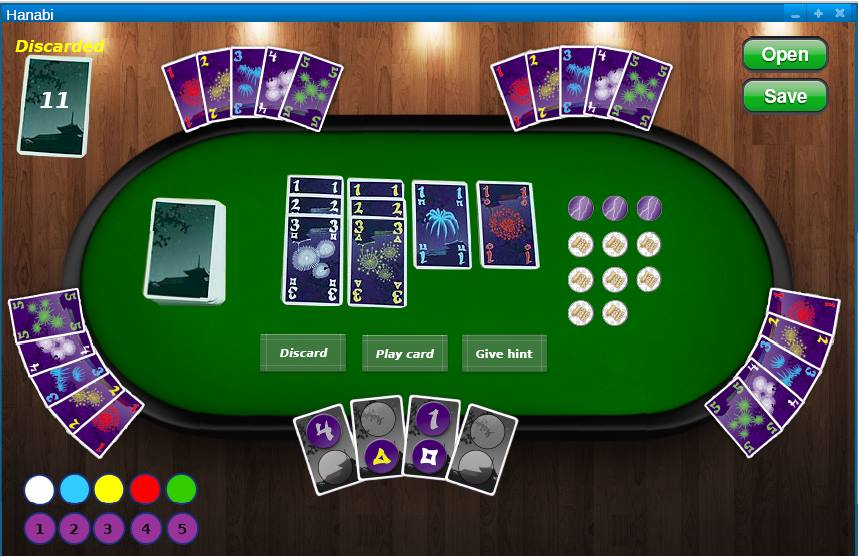
\includegraphics[scale = 0.4]{ihm.jpg}
\caption{Prototype d'interface graphique sur lequel on se base pour notre implémentation.}
\end{figure}

\subsection{Besoins non fonctionnels}

L’intelligence artificielle doit décider de son prochain coup en un temps limité afin que la partie se déroule normalement. Il est donc indispensable que les IAs soient efficaces et optimisées. 

{\normalfont Nous avons réflechi à plusieurs possibilités pour les IAs :}

\begin{itemize}
    \item {\bfseries Une IA simple} : cette IA joue d'une manière basique: elle joue une carte valide si possible (quand elle connaît la carte, et elle peut être posée), sinon, elle donne des indices aléatoires tant que des jetons sont disponibles, dans le cas contraire elle défausse une carte (en priorité les cartes déjà posées ou les cartes sans indices).
    \item {\bfseries Une IA sans risque} : cette IA ne joue des cartes que quand elle les connaît. Dans le cas contraire, elle évaluera s'il vaut mieux défausser une carte ou de donner un indice et lequel.
    \item {\bfseries Une IA qui prend des risques} : cette IA est moins adverse au risque. En utilisant une heuristique, elle évalue les probabilité de réussite des différentes actions possible et choisi le meilleur coup. 
    \item {\bfseries Une IA omnisciente} : cette IA connaît toutes les cartes (même les siennes), elle se concentre donc sur les priorités entre les différents coups possibles (jouer une carte qu'on connaît, défausser des cartes pour gagner des jetons <<indice>> ou donner des indices aux autres joueurs) 
\end{itemize}


\subsection{Critères d'acceptabilité du produit}

Notre but est de simuler un jeu entre deux ou plusieurs humains, en utilisant des IAs. Nous avons donc besoin d’avoir des intelligences artificielles efficaces qui ne prennent pas trop de temps pour calculer leur prochain coup. Nos critères d’acceptabilité par rapport aux intelligences artificielles sont donc :

\begin{itemize}
    \item De permettre à l’utilisateur de jouer une partie de Hanabi sans devoir attendre trop longtemps pour son tour.

    \item L’intelligence artificielle est considérée comme efficace si elle atteint systématiquement un score entre 20 et 25 (le score maximum possible) en ne jouant qu'entre des IAs avec la même stratégie.
\end{itemize}

Nous voulons aussi que le jeu soit facile et simple à jouer pour le joueur humain, donc une interface claire et compréhensible est indispensable. Il faut que toute personne soit capable de s’en servir. Nous voulons aussi avoir au moins une IA qui joue de façon réaliste plutôt que d'essayer de faire un score maximal.

\section{Déroulement du projet}

\subsection{Planification}

{\bfseries Février} :
\begin{itemize}
    \item Cahier des charges à rendre fin Février
\end{itemize}

{\bfseries Mars} :
\begin{itemize}
    \item 7 mars - Première IA basique. Elle ne joue ses cartes que quand elle les connaît et sait qu'elles sont valides. Sinon elle joue d'une manière aléatoire mais non risquée.
    \item 20 mars - Une meilleure IA, avec une fonction d'évaluation mais qui joue sans risque.
    \item 20 mars - Une première interface graphique.
\end{itemize}

{\bfseries Avril} :
\begin{itemize}
    \item 15 avril - Toutes les IAs terminées avec juste des petites modifications à faire.\\
\end{itemize}

{\bfseries Mai} :
\begin{itemize}
    \item 1 mai - Première version du rapport final
    \item 9 mai - Le rapport complet du projet ainsi que le code doivent être rendus
    \item 25 mai - Soutenance du projet
\end{itemize}
    

\subsection{Documentation}

Le logiciel doit être accompagné d’un document expliquant les règles du jeu, ainsi que d’un manuel d’utilisation. Le code sera accompagné d'une Javadoc pour décrire le fonctionnement de notre code. Il y aura également un rapport sur le déroulement du projet, expliquant en détail les raisonnements utilisés.

\subsection{Ressources}

Il y a plusieurs équipes qui ont déjà développé Hanabi en Java. Leurs projets sont disponibles sur Github et peuvent nous servir comme exemple. Nous pouvons nous inspirer de leurs interfaces et aussi de leurs intelligences artificielles.


{\bfseries GitHub Hanabi} :\\
https://github.com/jason17055/play-hanabi\\
https://github.com/kazocsaba/Hanabi



\end{document}
